%-- coding: UTF-8 --
\documentclass{gjm_hw}

\usepackage{showcode}
\usepackage{lipsum}

% \title{gjm-作业通用模板} % 不使用 title 
\author{gjm}
\date{Feb\ 24}
\setSemaster{Spring 2022}
\setCourse{算设}
\setAssignment{Hw 1}
\setSchoolId{2020019999}
\setContactInfo{gjm20@mails.tsinghua.edu.cn}

\begin{document}

  \maketitle
  
  \firstsection{标题左对齐}
    第一个section使用\code{$\backslash firstsection$},避免切换到新的一页;后续使用\code{$\backslash section$},会自动从新的一页开始section。
    \subsection{子标题也左对齐}
      \lipsum[1]
      \subsubsection{子子标题也左对齐}
        \lipsum[2]
    \subsection{展示带圈字符}
      \foreach \i in {1,2,...,20}{\circled{\i}\ }, \circled{Hello, world.}
  
  \section{问题列表}
  整个文档使用同一个问题计数器,当然,也可以使用\code{$\backslash$setcounte\{ProblemCounter\}\{1\}}重设计数。
  
  \subsection{双列问题列表}
    \begin{multicols}{2} % 两列开始
    \begin{problem}
    \ptitle{\par Prove: $2n+\Theta\left(n^{2}\right)=\Theta\left(n^{2}\right)$}{}
    \begin{solution}
    \vspace{-0.5cm}
    \begin{flalign*}
      & \because \text{根据$\Theta$定义} &&\\
      & \therefore \exists n_0,c_1,c_2,\ s.t.\ \forall n > n_0,\ c_1n^2 \le \Theta(n^2) \le c_2n^2&& \\
      & \therefore c_1+2/n \le \frac{2n+\Theta(n^2)}{n^2} \le c_2+2/n && \\
      & \therefore c_1 \le \frac{2n+\Theta(n^2)}{n^2} \le c_2+3 && \\
      & \therefore c_1n^2 \le 2n+\Theta(n^2) \le (c_2+3)n^2 && \\
      & \therefore 2n+\Theta(n^2) = \Theta(n^2) &&
    \end{flalign*}
    \end{solution}
    \end{problem}
    
    \begin{problem}
    \ptitle{\par Prove: $\Theta(g(n)) \cap o(g(n))=\emptyset$}{}
    \begin{solution}
    \vspace{-0.5cm}
    \begin{flalign*}
      & \forall f \in \Theta(g),\ \exists c_2,n_0,\ 
          s.t.\ \forall n > n_0,\ g \le c_2f && \\
      & \text{若}\ f \in o(g), \text{则}\ \forall c,\ \exists n_1,\ 
          s.t.\ \forall n > n_1,\ cf<g && \\
      & \text{这与} f \in \Theta(g) \text{矛盾} && \\
      & \therefore \Theta(g(n)) \cap o(g(n))=\emptyset &&
    \end{flalign*}
    \end{solution}
    \end{problem}
    在这里使用\code{$\backslash columnbreak$}强制换栏
    \columnbreak % 强制换栏
    
    \begin{problem}
    \ptitle{\par Prove: $\Theta(g(n)) \cup o(g(n)) \neq O(g(n))$}{\par \hfill Ref to book.}
    \begin{solution}
    直观理解三个符号:
    \begin{flalign*}
      \Theta(g) &\iff f/g \quad \text{有界, 且下确界>0} \hfill && \\
      o(g) &\iff f/g \quad \to 0  \hfill&& \\
      O(g) &\iff f/g \quad \le const &&
    \end{flalign*}
    \begin{flalign*}
      & \therefore \text{设}\ g = n^2,\ f = (1+(-1)^n)n^2 && \\
      & \text{此时},\ f = O(g),\ \text{但是} f \ne \Theta(g) \text{且} f \ne o(g) &&
    \end{flalign*}
    \end{solution}
    \end{problem}
    
    \begin{problem}
    \ptitle{\par Prove: $\max (f(n), g(n))=\Theta(f(n)+g(n))$}{}
    \begin{solution}
    \vspace{-0.5cm}
    \begin{flalign*}
      & \because f, g \ge 0 && \\
      & \therefore max(f,\ g) \le f+g \le 2max(f,\ g) && \\
      & \therefore c_1 = 1,\ c_2 = 2 && \\
      & \therefore \max (f(n), g(n))=\Theta(f(n)+g(n)) &&
    \end{flalign*}
    \end{solution}
    \end{problem}
    \end{multicols}
  
  \clearpage
  
  \subsection{单列问题列表}
    \setcounter{ProblemCounter}{1}
    \begin{problem}
    \ptitle{Relative asymptotic growths}{CLRS, P61, 3-2}
    Indicate, for each pair of expressions $(A, B)$ in the table below, whether $A$ is $O, o$, $\Omega, \omega$, or $\Theta$ of $B$. Assume that $k \geq 1, \epsilon>0$, and $c>1$ are constants. Your answer should be in the form of the table with "yes" or "no" written in each box. \par
    \begin{solution}
    \begin{figure}[H]
        \centering
        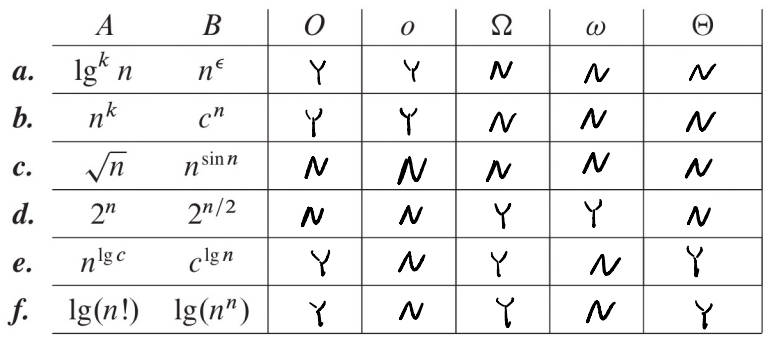
\includegraphics[height=4cm]{images/3-2.jpg}
    \end{figure}
    \end{solution}
    \end{problem}
    
    \begin{problem}
    \ptitle{Ordering by asymptotic growth rates}{CLRS, P61, 3-3}
    a. Rank the following functions by order of growth; that is, find an arrangement $g_{1}, g_{2}, \ldots, g_{30}$ of the functions satisfying $g_{1}=\Omega\left(g_{2}\right), g_{2}=\Omega\left(g_{3}\right), \ldots$, $g_{29}=\Omega\left(g_{30}\right)$. Partition your list into equivalence classes such that functions $f(n)$ and $g(n)$ are in the same class if and only if $f(n)=\Theta(g(n))$.
    $\begin{array}{cccccc}\lg \left(\lg ^{*} n\right) & 2^{\lg ^{*} n} & (\sqrt{2})^{\lg n} & n^{2} & n ! & (\lg n) ! \\ \left(\frac{3}{2}\right)^{n} & n^{3} & \lg ^{2} n & \lg (n !) & 2^{2^{n}} & n^{1 / \lg n} \\ \ln \ln n & \lg ^{*} n & n \cdot 2^{n} & n^{\lg \lg n} & \ln n & 1 \\ 2^{\lg n} & (\lg n)^{\lg n} & e^{n} & 4^{\lg n} & (n+1) ! & \sqrt{\lg n} \\ \lg ^{*}(\lg n) & 2^{\sqrt{2} \lg n} & n & 2^{n} & n \lg n & 2^{2^{n+1}}\end{array}$\par
    \vspace{1em}
    b. Give an example of a single nonnegative function $f(n)$ such that for all functions $g_{i}(n)$ in part (a), $f(n)$ is neither $O\left(g_{i}(n)\right)$ nor $\Omega\left(g_{i}(n)\right)$ \par
    \begin{solution}
    
    a. $a > b$ 表示 $a = \Omega(b)$, $a = b$ 表示 $a = \Theta(b)$。
      顺序为:$2^{2^{n+1}}\ > \ 2^{2^n}\ >\ (n+1)!\ >\ n!\ >\ e^n\ >\ 
      n\cdot 2^n\ >\ 2^n\ >\ (3/2)^n\ >\ (\lg n)^{\lg n}\ =\ n^{\lg\lg n}\ >\ 
      (\lg n)!\ >\ n^3\ >\ 
      n^2\ =\ 4^{\lg n}\ >\ n\ln n\ =\ \lg n!\ >\ n\ =\ 2^{\lg n}\ >\ 
      (\sqrt{2})^{\lg n}\ >\ 2^{\sqrt{2\lg n}}\ >\ \lg^2 n\ >\ 
      \ln n\ >\ \sqrt{\lg n}\ >\ \ln\ln n\ >\ 2^{\ln^* n}\ >\ \lg^*n\ =\ \lg^*(\lg n)\ >\ \lg(\lg^* n)
      \ >\ n^{1/\lg n}\ =\ 1$
    
    b. $f(n)=\left(1+(-1)^{n}\right) n$
    \end{solution}
    \end{problem}
    
  \section{绘制图、树}
  
    如果要绘制图、树,使用\code{LuaLaTeX}编译,否则使用\code{XeLaTeX}编译,要快一些。
    
    \begin{center}
    \begin{tikzpicture}
    \graph[tree layout, nodes={draw,circle}]{
      1--{2,3,4,5},
      2--{6,7},
      5--8--9->{10, 11},
      6--10
    };
    \foreach \x in {5, 8, 9, 11} \node at (\x)[right=1em]{$v_{\x}$};
    \end{tikzpicture}
    \end{center}
    
    更多例子可见https://texample.net/
    
  \section{伪代码示意}
    \begin{algorithm}[H]
    \caption{Subproblem Optimize} \label{subpro-opt}
    \begin{algorithmic}[1]
    \If{$r-l \le 30$}
        \State sort p.pointlist by a specific sort algorithm
        \State calculate minimal distance brutely here
        \State \Return minimal distance
    \ElsIf{$l \ge r-1$}
        \State \Return INF
    \EndIf
    \end{algorithmic}
    \end{algorithm}
    
    引用代码使用 \refalg{subpro-opt}。如果要允许代码块换行,使用breakablealgorithm代替algorithm。

  \section{代码渲染}
  
  这里展示文档内代码渲染功能,支持内插代码和从文件读取代码。
  
  \begin{lstlisting}[language=C++, title=Example Code 1]
// This is an example of code block.
// Language: C++
#include <iostream>
using namespace std;
int main ()
{
	cout << "Hello World!" << endl;
	return 0;
}
  \end{lstlisting}
	
  \lstinputlisting[language=python, title=Load from file]{ExpGen.py}

\end{document}